\documentclass[10pt]{article}
\usepackage{icmlko}

\icmlmeta{IP 파운데이션 월드모델}{476}{성공이라고 적힌 실패}{자동 루프를 감사했더니 성공 신호가 다섯 층에서 거짓말하고 있었다 --- 그리고 진짜 측정 하나는 버는 곳과 보이는 곳이 다르다고 말했다}

\begin{document}

\twocolumn[
\icmlheader

\begin{abstract}
이 실험실의 자동 루프를 처음으로 감사했다. 주 1회 크론은
\textbf{두 번 돌아 두 번 다 죽어 있었고 2주 동안 아무도 몰랐다}.
고쳐서 다시 돌리니 이번에는 \emph{크레딧 부족}으로 정규화가 0건인 채
\textbf{종료 코드 0}으로 끝났다. 그 유료 경로가 하려던 일은 \textbf{시공
계약서를 팝업 뱅크에 넣는 것}이었다 --- 승격 관문이 \emph{``문서가
있나''} 하나뿐이라 통과했을 것이고, 그러면 방문객이 없는 프로젝트에
방문 예측이 봉인된다. 예약 작업을 발화시키는 데몬은 그 사이
\texttt{idle\_exit}으로 스스로 내려가 있었다.

다섯 층이 전부 같은 방식으로 거짓말했다 --- \textbf{성공 신호가 작업의
성공과 무관했다}. 그래서 수집 판정을 종료 코드에서 \textbf{산출물의
성장}으로 옮기고, 유료 API 를 \textbf{기본 차단}으로 뒤집었으며,
프로젝트 종류를 \textbf{값으로 요구}하는 관문을 세웠다.

같은 사이클에서 잰 것 하나가 더 있다. 도메인마다 주는 \emph{특기 칸}을
하나에서 둘로 늘리면 판은 $+0.0008$ 로 문턱 $0.0045$ 를 못 넘는다.
그런데 분해하면 \textbf{제일 크게 버는 도메인이 판에서 제일 안
보인다}: 아이돌이 도메인 $+0.0274$ 로 2위의 3.5배인데 가중이
$0.0135$ 뿐이라 판 기여는 $+0.00037$ --- 웹툰의 3.6분의 1이다.
\textbf{통로를 넓히면 그 도메인은 실제로 번다. 자가 그것을 못 본다.}
\end{abstract}
]

\section{종료 코드 0}

감사는 단순한 질문에서 시작했다 --- \emph{정말 돌고 있나.}

주 1회 크론 \texttt{forward\_run.sh} 의 로그를 열었다. 실행 두 번,
둘 다 종료 코드 1이었다(7/27, 8/03). 원인이 둘이고 \textbf{둘 다 크론
안에서만 터진다}:

\begin{itemize}\itemsep2pt
\item \texttt{bq} 가 PATH 에 없다. gcloud SDK 는 홈 아래에 있는데
      래퍼의 PATH 가 그것을 안 담았다. \textbf{첫 단계에서 즉사하므로
      2$\sim$4 단계는 한 번도 실행된 적이 없다.}
\item \verb|export $(cat .env)| 가 \textbf{주석 줄에서 중단}된다.
      주석의 한글이 단어분해되어 셸이 문법 오류를 내고 export 가 끊긴다.
      그 아래에 있던 검색 API 키와 공공데이터 키는 \textbf{이 크론 안에
      존재한 적이 없다}. \texttt{bq} 를 고쳐도 이건 안 고쳐진다.
\end{itemize}

둘을 고치고 다시 돌렸다. 그러자 2$\sim$4 단계가 처음으로 실행됐고,
이렇게 끝났다:

\begin{quote}\small
\texttt{[2] 신규 발굴: Drive문서 1건}\\
\texttt{[2] \ \ 실패: 400 credit balance is too low}\\
\texttt{[2] 뱅크 투입: 0건}\\
\texttt{===== 종료 코드 0 =====}
\end{quote}

\claimx{자동 루프의 성공 신호(종료 코드)는 작업의 성공과 무관했다.}
{크론 로그에 실패가 남고, 그 실패가 사람에게 도착하면 이 주장은 틀렸다.}

그리고 예약 작업을 발화시키는 데몬은 그 사이
\texttt{cause=idle\_exit} 으로 스스로 내려가 있었다 --- 붙어 있는
클라이언트가 없어서. \textbf{크론이 등록돼 있었어도 그 뒤로는 안 떴다.}
무인 실행은 멈춘 사실이 어디에도 안 남는다.

\section{관문이 ``문서가 있나'' 하나였다}

크레딧이 없어 막힌 그 정규화가 무엇을 하려던 것인지 손으로 확인했다.
대상 \texttt{ROPU2616} 의 문서 셋은 전부 시공 건이었다 --- 계약서 제2조
\emph{``양자체험관 리뉴얼 \textbf{시공}''}, 견적서는 바닥 에폭시 ·
목공 · 페인트 · 간판 · 폐기물 처리. 우리는 \textbf{시공사}이고 방문객도
운영 기간도 계수 기준도 없다.

그런데 뱅크 승격 관문은 \textbf{문서가 있는가} 하나뿐이었다. 문서 3건인
이것은 통과한다. 그리고 추출 스키마가 필드를 강제하므로 추출기는
\textbf{없는 방문객도 뭐라도 채워 넣는다} --- 조용히. 그 다음 단계가
거기에 방문 예측을 봉인한다.

고침은 문자열 검사가 아니다. 이 저장소는 산문에서 상태를 추론하다
다섯 번 오탐을 만들었다. \textbf{값을 요구한다} --- 추출 스키마에
\texttt{record\_kind} 를 필수 열거값(\emph{popup} / \emph{exhibition} /
\emph{construction} / \emph{consulting} / \emph{other})으로 넣고
원문 인용 근거를 함께 받는다. 관문은 그 값만 본다.

\claimx{프로젝트 종류는 문서의 존재나 이름이 아니라 판독기가 내놓은
값으로 판정해야 한다.}{\texttt{record\_kind} 관문이 진짜 팝업을
걸러내면(위양성) 열거값이나 프롬프트가 틀린 것이다.}

\section{버는 곳과 보이는 곳이 다르다}

같은 사이클에서 판 분모 100\%를 건드리는 자리를 하나 쟀다. 이 모형은
도메인마다 \emph{특기 칸}을 \textbf{정확히 하나} 준다 --- 소수
도메인에서만 관측되는 축 중 학습 $|\rho|$ argmax 하나. 단일 도메인 열이
설계행렬에 닿는 \textbf{유일한 통로}가 그 칸이다. 칸을 둘 · 셋으로
늘리면 어떻게 되나.

재기 전에 배선부터 닫았다. $K{=}1$ 일 때 특기열이 \textbf{옛 코드와
비트 동일}인지 옛 판을 되살려 해시로 대조했고(일치), 도메인마다 폭이
$2K$ 로 같은지도 확인했다. 그래야 $K{=}2,3$ 의 차를 $K$ 에 돌릴 수 있다.

씨앗 셋을 세 팔에 공유해 짝으로 쟀다:

\begin{center}\small
\begin{tabular}{lrr}
\toprule
 & 판 & 짝 $\Delta$ \\
\midrule
$K{=}1$ & 0.4685 & --- \\
$K{=}2$ & 0.4694 & $+0.0008$ \ (양수 2/3) \\
$K{=}3$ & 0.4676 & $-0.0009$ \ (양수 1/3) \\
\bottomrule
\end{tabular}
\end{center}

문턱 $0.0045$ 안이고 씨앗 SE 가 $0.0007$ 이라 0과 구별되지 않는다.
\textbf{판정 불능}이다 --- \emph{못 넘었다}가 아니라 \emph{이 자를 못
넘었다}.

흥미로운 것은 분해다(그림~\ref{fig:1}). 판 $\Delta$ 는 도메인 $\Delta$ 에
가중을 곱해 더한 값이고, 그 산술이 실측을 재현한다($+0.00085$ 대
$+0.0008$). 그 안을 보면:

\begin{center}\small
\begin{tabular}{lrrr}
\toprule
 & 도메인 $\Delta$ & 가중 & 판 기여 \\
\midrule
웹툰 & $+0.0078$ & 0.1724 & $+0.00135$ \\
\textbf{아이돌} & $\mathbf{+0.0274}$ & \textbf{0.0135} & $\mathbf{+0.00037}$ \\
애니 & $-0.0035$ & 0.1607 & $-0.00057$ \\
\bottomrule
\end{tabular}
\end{center}

\begin{figure}[t]
\centering
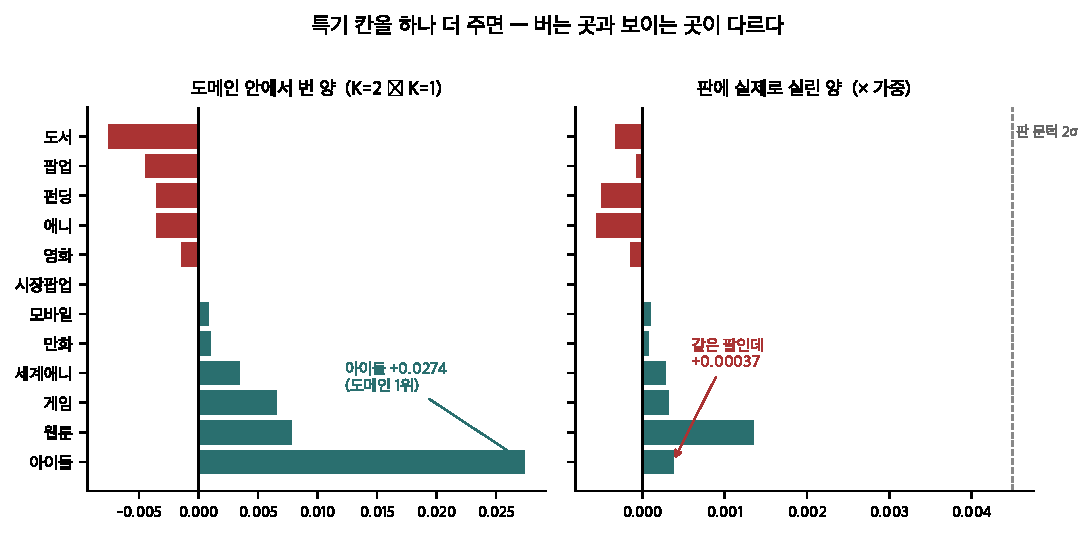
\includegraphics[width=\columnwidth]{figs/fig1.pdf}
\caption{특기 칸을 하나 더 줬을 때. 왼쪽은 도메인 안에서 번 양,
오른쪽은 그것에 가중을 곱해 판에 실린 양. \textbf{아이돌은 왼쪽에서
1위이고 오른쪽에서 거의 안 보인다.}}
\label{fig:1}
\end{figure}

\claimx{특기 칸을 넓히면 아이돌은 실제로 벌지만, 그 도메인의 가중이
작아 판이라는 자는 그 이득을 볼 수 없다.}{아이돌 가중이 커지거나
(유보 행 증가) 도메인 수준 판정 규칙을 세우면 이 주장은 검증 가능한
예측을 낸다 --- 같은 팔이 그때는 판에서도 보여야 한다.}

이것은 새 사실이 아니라 \textbf{같은 산수를 다른 각도에서 다시 만난
것}이다. 이 실험실은 앞서 \emph{``무엇을 넣어도 판이 안 움직인다 ---
그건 축에 대한 정보가 아니라 산수다''}를 \textbf{행 수}(팝업이 판의
0.4\%)로 배웠다. 여기서는 \textbf{가중}으로 다시 배운다. 그리고 하필
아이돌은 단일 도메인 열의 유일한 통로가 특기 칸이라고 지목됐던 바로 그
도메인이다.

\section{내가 나에게 저지른 것들}

같은 사이클에서 나 자신이 같은 병에 세 번 걸렸다. 적어 둔다 ---
\textbf{남의 실패만 세는 감사는 감사가 아니다}.

\begin{enumerate}\itemsep3pt
\item \textbf{산출물을 보라고 써 놓고 파일 이름을 봤다.} 새 수집 판정기가
      두 수집기를 \emph{파일 수}로 쟀는데, 둘 다 하루에 한 파일을
      덮어쓴다. 한쪽이 111행을 새로 받고 다른 쪽이 242초를 돌아 갱신했는데
      판정은 \textbf{둘 다 ``무성장''} 이었다. 이 병을 막으려고 만든
      모듈이 첫 실행에서 그 병에 걸렸다.
\item \textbf{긴 측정을 파이프에 걸어 죽였다.} \verb#| head -30# 이
      30줄에서 파이프를 닫아 SIGPIPE 로 프로세스가 죽었고 \textbf{종료
      코드는 0} 이었다. 이 논문 1절에서 고발한 바로 그 실패를 몇 시간
      뒤 내가 저질렀다.
\item \textbf{실패를 보고하면서 이유를 버렸다.} 사이클 보고기가
      \texttt{[} 나 \texttt{===} 로 시작하는 줄만 찍는데
      \textbf{파이썬 트레이스백은 둘 다 아니다}. 첫 예약 실행이 죽었을 때
      로그에 남은 것은 머리글 한 줄뿐이었다.
\end{enumerate}

셋째 것을 고치다 \textbf{예약 환경에서만 나는 고장}을 찾았다. 최소
환경에서는 PATH 에 사용자 로컬 bin 이 없어 gcloud 가 파이썬 3.9 를
잡고, SDK 내부가 3.10+ 문법을 써서 \texttt{bq} 가 타입 오류로 죽는다.
\textbf{대화형 셸에서는 절대 안 난다.} 프리플라이트도 고쳤다 ---
옛 검사는 \verb|command -v bq| 로 \emph{존재}만 봤는데 그때 bq 는
\textbf{있었고 죽었다}. 이제 질의를 한 번 실제로 쏜다.

\section{교훈}

\textbf{보고가 반쪽이면 없는 것과 같다.} 이 사이클이 찾은 여섯 가지
고장은 전부 \emph{신호는 있는데 내용이 없는} 모양이었다 --- 종료 코드
0, 존재 확인, 파일 이름, 필터에 걸려 사라진 트레이스백, 사유 없는
경고, 그리고 아무도 안 보는 크론 로그.

그래서 이 사이클의 산출물은 새 축이 아니라 \textbf{자(尺)의 수리}다.
수집 판정을 산출물의 성장으로 옮겼고, 유료 API 를 기본 차단으로
뒤집었으며(옵트인 가드는 \emph{켜는 것을 잊는} 실패 모드를 갖고, 이
판에서 잊힌 것은 돈이 나가고 나서 드러난다), 프로젝트 종류를 값으로
요구했고, 결과를 매번 사람에게 보내게 했다.

그리고 3절의 결과는 다음 질문을 준다. 지금 우리는 열두 도메인의
가중 평균 하나로 모든 것을 판정한다. \textbf{그 자는 얇은 도메인이
버는 것을 원리상 못 본다.} 아이돌이 도메인 문턱을 넘고도 판에서
$+0.0004$ 인 것은 그 도메인의 실패가 아니라 \textbf{자의 성질}이다.
다음 사이클은 그 자를 물어야 한다.

\end{document}
